
\vspace{-1em}
\begin{center}
\begin{minipage}{0.6\textwidth}
\begin{abstract}
This report presents a pipeline for detecting and retrieving fashion items from images using a fine-tuned YOLOS object detection model and a ResNet50-based similarity search. The approach involves detecting clothing items, cropping them, extracting features, and retrieving similar items from a precomputed dataset.
\end{abstract}
\end{minipage}
\end{center}

Fashion item detection and retrieval are crucial for applications like e-commerce and digital wardrobe management. Leveraging transformer-based models like YOLOS and convolutional neural networks like ResNet50 enables accurate detection and efficient retrieval of fashion items.

\section*{Problem Statement}

In today's digital age, fashion trends are often driven by celebrities, influencers, and social media figures. We frequently come across images of individuals wearing outfits we admire—be it in movies, on social media platforms, or during public appearances. These images serve as inspiration for our personal fashion choices.

However, translating that inspiration into actual purchases poses a challenge. The average user lacks the tools to identify, locate, and purchase similar clothing items. Manually searching for the same or similar products on e-commerce platforms can be time-consuming, inaccurate, and often frustrating.

Wouldn't it be transformative if users could simply upload an image of their fashion inspiration—such as a celebrity wearing a specific outfit—and the e-commerce platform could automatically detect and retrieve similar clothing items from its inventory?

This project proposes a solution that combines object detection and visual similarity search to power a feature for modern e-commerce platforms. By detecting fashion items in user-uploaded images and retrieving visually similar items available in the store, we can create a seamless bridge between inspiration and purchase. Such a system not only enhances user experience but also opens new avenues for personalization and sales conversion in the fashion retail industry.

\section*{Datasets}

Two distinct datasets were used in the development of this system, each serving a different purpose in the workflow:

\begin{itemize}
    \item \textbf{Fashionpedia Dataset}: This dataset, available on Hugging Face at \url{https://huggingface.co/datasets/detection-datasets/fashionpedia}, was used to fine-tune the YOLOS object detection model. Fashionpedia contains richly annotated fashion images with 46 clothing and accessory categories and pixel-level segmentation, making it ideal for training object detectors in the fashion domain.

    \item \textbf{Fashion Product Images Dataset}: Sourced from Kaggle at \url{https://www.kaggle.com/datasets/paramaggarwal/fashion-product-images-dataset}, this dataset serves as a simulated store catalog. It contains a large number of product images that are used for feature extraction and similarity search. Although the dataset lacks fine-grained textual labels (e.g., "red t-shirt", "striped jeans"), it is sufficient for the visual matching task required in this application, where the images themselves act as dummy inventory items in the store.
\end{itemize}



\section*{Model Architecture}

\subsection*{YOLOS for Object Detection}
YOLOS (You Only Look at One Sequence) is a transformer-based model adapted for object detection tasks. Fine-tuning YOLOS on fashion datasets allows for precise detection of various clothing items. The model processes images to predict bounding boxes and class probabilities for detected objects.

\subsection*{ResNet50 for Feature Extraction}
ResNet50, a deep convolutional neural network, is employed to extract features from cropped images of detected fashion items. By removing the top classification layer and adding a Global Max Pooling layer, the model outputs feature vectors representing the visual characteristics of each item.

\section*{Workflow}

The following outlines the workflow of the system that enables users to find similar clothing items from an e-commerce catalog based on an input image:

\begin{enumerate}
    \item \textbf{Image Upload:} The user uploads an image of a person (e.g., a celebrity or influencer) wearing clothes they admire.

    \item \textbf{Object Detection:} The image is processed using a fine-tuned YOLOS model which identifies and classifies different fashion items within the image.

    \item \textbf{Category Selection:} Detected clothing items are visually presented with bounding boxes. The user selects a specific category of interest (e.g., \textit{pants}, \textit{jacket}).

    \item \textbf{Cropping:} The selected clothing item is cropped from the original image using its bounding box for isolated feature extraction.

    \item \textbf{Feature Extraction:} A ResNet50 model (without the classification head) with GlobalMaxPooling is used to extract feature vectors from the cropped image. This vector represents the visual characteristics of the item.

    \item \textbf{Similarity Search:} The extracted feature vector is compared against a precomputed database of features from the store's catalog using a \texttt{Nearest Neighbors} model. The closest matches are retrieved based on visual similarity.

    \item \textbf{Result Display:} The top visually similar clothing items are displayed to the user, enabling quick browsing and purchase options for similar fashion items.
\end{enumerate}

It can be summarized in teh following diagram:

\begin{figure}[H]
  \centering
    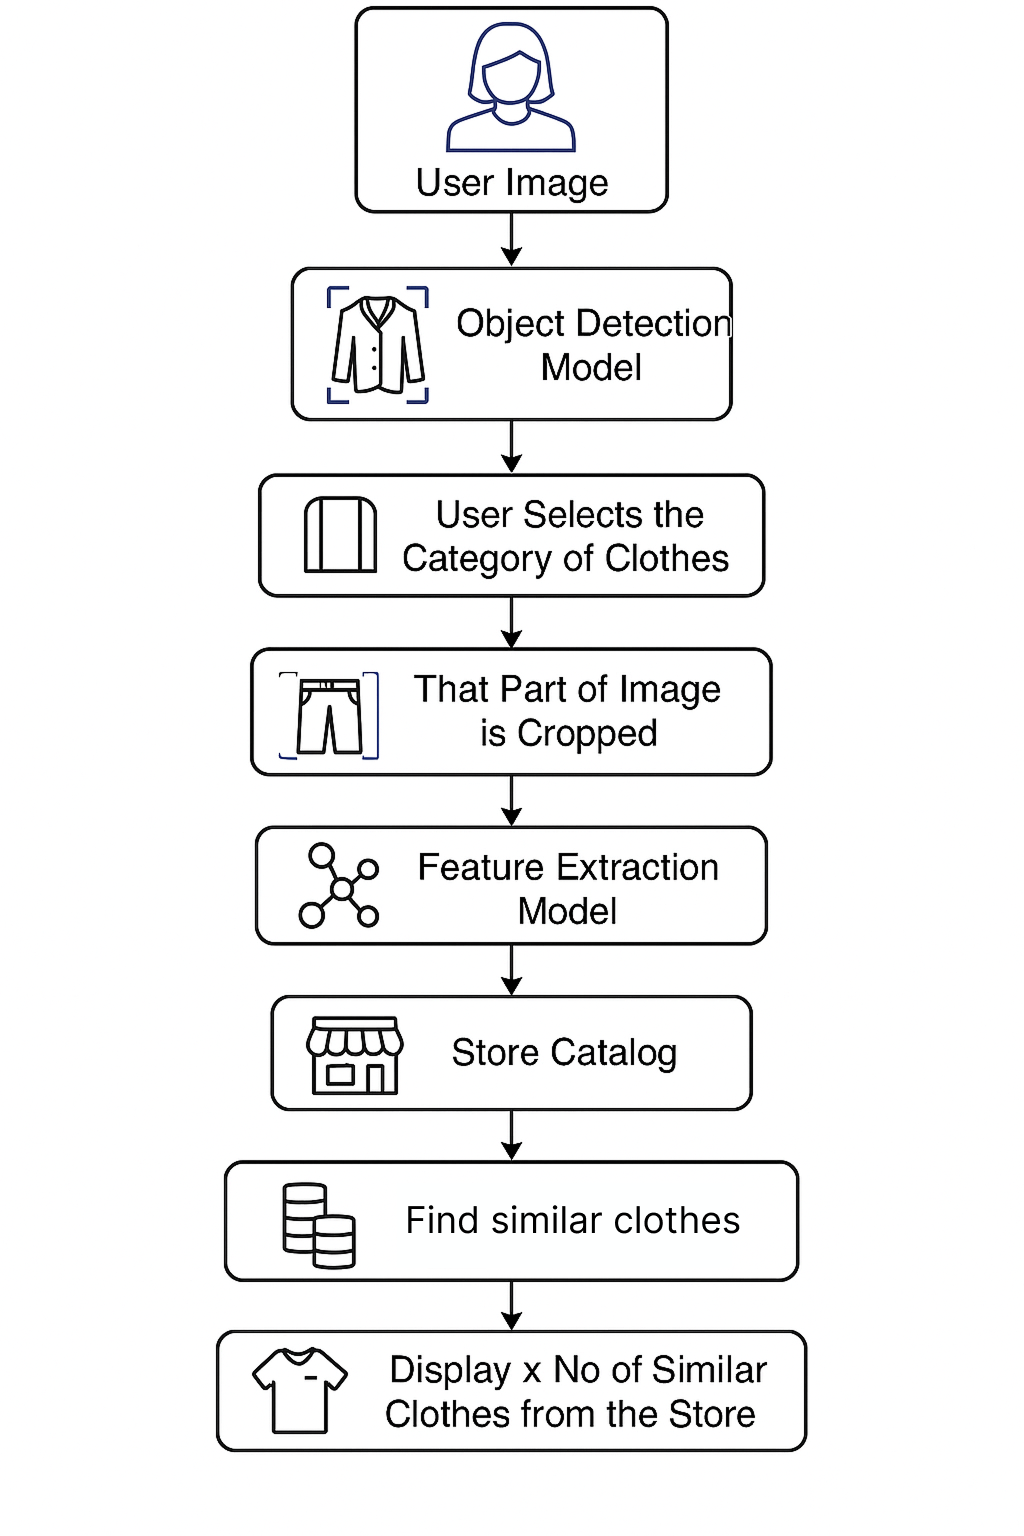
\includegraphics[width=0.35\textwidth]{images/workflow.png}
  \end{figure}

\section*{Methodology}

\subsection*{Data Acquisition and Preprocessing}
An input image is obtained from a specified URL and processed to ensure it has three channels (RGB). The YOLOS feature extractor converts the image into a suitable format for the model.

\subsection*{Object Detection and Cropping}
The YOLOS model predicts bounding boxes and class labels for objects in the image. Bounding boxes corresponding to the specified category (e.g., "pants") are used to crop the relevant portions from the original image.

\subsection*{Feature Extraction}
Each cropped image is resized to $224 \times 224$ pixels and passed through the modified ResNet50 model to obtain a normalized feature vector.

\subsection*{Similarity Search}
A Nearest Neighbors model is trained on precomputed feature vectors from a dataset of fashion items. For each cropped image, the model retrieves the top 5 most similar items based on Euclidean distance in the feature space.

\section*{Results}

Here is how the pipeline works in practice. The following images illustrate the process of detecting clothing items, cropping them, and retrieving similar items.


\begin{figure}[H]
    \centering
    \begin{subfigure}[b]{0.3\textwidth}
        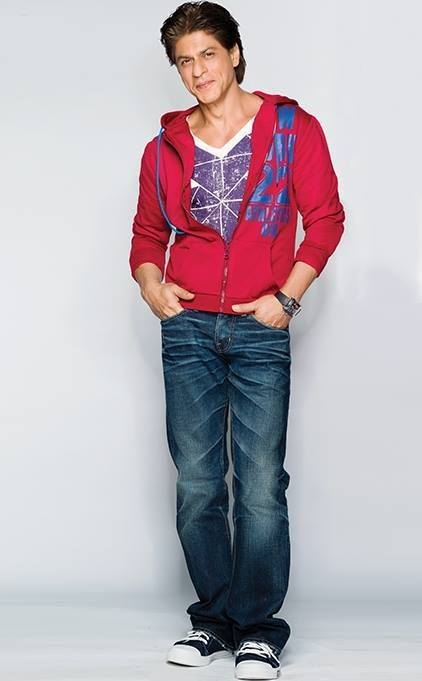
\includegraphics[width=\textwidth]{images/og_image.png}
        \caption{Original Image}
    \end{subfigure}
    \begin{subfigure}[b]{0.3\textwidth}
        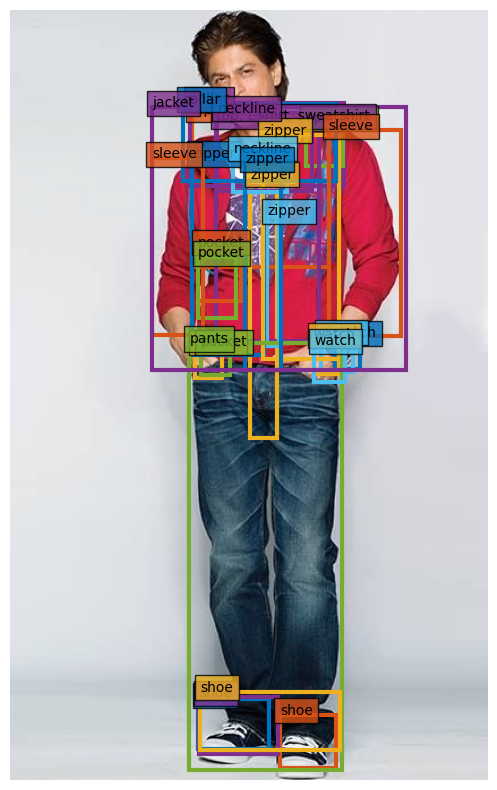
\includegraphics[width=\textwidth]{images/detected_imgae.png}
        \caption{Clothes Detected}
    \end{subfigure}
    \begin{subfigure}[b]{0.2\textwidth}
        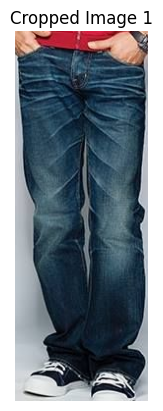
\includegraphics[width=\textwidth]{images/cropped_image.png}
        \caption{Cropped only Pants}
    \end{subfigure}
\end{figure}

\begin{figure}[H]
    \centering
    \begin{subfigure}[b]{0.19\textwidth}
        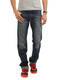
\includegraphics[width=\textwidth]{images/output1.jpeg}
        \caption{Match 1}
    \end{subfigure}
    \begin{subfigure}[b]{0.19\textwidth}
        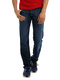
\includegraphics[width=\textwidth]{images/output2.jpeg}
        \caption{Match 1}
    \end{subfigure}
    \begin{subfigure}[b]{0.19\textwidth}
        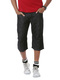
\includegraphics[width=\textwidth]{images/output3.jpeg}
        \caption{Match 1}
    \end{subfigure}
    \begin{subfigure}[b]{0.19\textwidth}
        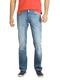
\includegraphics[width=\textwidth]{images/output4.jpeg}
        \caption{Match 1}
    \end{subfigure}
    \begin{subfigure}[b]{0.19\textwidth}
        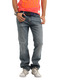
\includegraphics[width=\textwidth]{images/output5.jpeg}
        \caption{Match 1}
    \end{subfigure}
    \caption{Top 5 similar items for Cropped Image 1.}
    \label{fig:similar_items_1}
\end{figure}

\section*{Future Work}
While the current system lays the foundation for a powerful visual product recommendation engine, there are several avenues for improvement and extension:

\begin{itemize}
    \item \textbf{Web Integration:} Develop a user-friendly web interface where users can upload images and receive fashion recommendations instantly.
    \item \textbf{LLM Integration:} Integrate large language models to support natural language queries like "Show me similar red jackets" or "Find dresses worn by celebrities."
    \item \textbf{Mobile Application:} Create a mobile app for easy and on-the-go usage, leveraging device cameras and local caching.
    \item \textbf{Personalized Recommendations:} Incorporate user preferences, browsing history, and past purchases to refine suggestions.
    \item \textbf{Multi-clothing Detection:} Extend the pipeline to handle multiple clothing items simultaneously and generate multiple sets of suggestions.
    \item \textbf{Multimodal Search:} Combine visual search with textual filters like price, size, color, or material.
    \item \textbf{Faster Search Backend:} Replace brute-force nearest neighbors with FAISS indexing for faster and scalable similarity search.
    \item \textbf{Inventory Sync:} Automatically sync with store inventories to only recommend available products in real-time.
    \item \textbf{Social Sharing:} Allow users to share their finds with friends on social platforms for feedback and engagement.
\end{itemize}


\section*{Conclusion}
The integration of YOLOS for object detection and ResNet50 for feature extraction provides an effective pipeline for fashion item retrieval. This approach can be extended to various fashion categories and integrated into recommendation systems or virtual try-on applications.

\section*{References}
\begin{enumerate}
  \item You Only Look at One Sequence: Rethinking Transformer in Vision through Object Detection
  : \url{https://arxiv.org/abs/2106.00666}
\end{enumerate}